\section{Pre-Training}
Similar to GLM-4.5, the base model of GLM-5 goes through two stages: pre-training for general language and coding capacity, and mid-training for agentic and long-context capacity. We extend the training token budget for all the training stages of GLM-5, totaling 28.5 trillion tokens for the base model.

\subsection{Architecture}

\paragraph{Model size scaling.} GLM-5 scales to 256 experts and reduces its layer count to 80 to minimize expert parallelism communication overhead. This results in a 744B parameter model (40B active parameters), doubling the total size of GLM-4.5, which utilized 355B total and 32B active parameters.

\begin{table}[!ht]
    \small
    \centering
    \caption{Evaluation results for GQA-8 and variants of MLA.}
    \begin{tabular}{c|cccccccc}
        \toprule
        Dataset & Hellaswag & MMLU & C-Eval & RACE & BBH & GSM8K & HumanEval \\
        \midrule
        GQA-8 & 77.3 & 61.2 & 60.0 & 79.6 & \textbf{53.3} & \textbf{47.6} & \textbf{38.5} \\
        MLA & 77.3 & 61.5 & 59.7 & 77.8 & 48.9 & 46.2 & 33.5 \\
        MLA + Muon Split & \textbf{77.8} & \textbf{62.5} & \textbf{62.1} & \textbf{79.9} & 51.8 & 45.0 & 36.7\\
        MLA-256 + Muon Split & 77.4 & 62.0 & 59.9 & 79.6 & 51.3 & 47.5 & 36.6 \\
        \bottomrule
    \end{tabular}
    \label{tab:mla}
\end{table}

\paragraph{Multi-latent Attention.} By employing reduced key-value vectors, Multi-latent attention (MLA)~\cite{liu2024deepseekv2} matches the effectiveness of Grouped-Query Attention (GQA) but offers superior GPU memory savings and faster processing for long-context sequences.

However, in our experiments with Muon optimizer, we find that MLA with a 576-dimension latent KV-cache cannot match the performance of GQA with 8 query groups (denoted as GQA-8, 2048-dimension KV-cache). To overcome the performance gap, we propose an adaptation to the recipe of Muon optimizer in GLM-4.5.
In the original recipe, we apply matrix orthogonalization to the up-projection matrices $W^{UQ}, W^{UK}, W^{UV}$ for multi-head queries, keys, and values. Instead, we split these matrices into smaller matrices for different heads and apply matrix orthogonalization to these independent matrices. The method, denoted as Muon Split, enables projection weights for different attention heads to update at different scales. As shown in \Cref{tab:mla}, the method effectively improves the performance of MLA to match that of GQA-8. In practice, we also find that with Muon Split, the scale of attention logits of GLM-5 remains stable during pre-training without any clipping strategy.

Another disadvantage of MLA is its high computational cost during decoding. In decoding, MLA performs a 576-dimensional dot product, higher than the 128-dimensional computation of GQA. While the number of attention heads in DeepSeek-V3 is selected according to the roofline of H800~\cite{zhao2025insights}, it is inappropriate for other hardware. Given the Multi-head Attention (MHA) style of MLA during training and prefilling, we increase the head dimension from 192 to 256 and decrease the number of attention heads by 1/3. This keeps the training computation
and the number of parameters constant while decreasing the decoding computation. The variant, denoted as MLA-256 in \Cref{tab:mla}, matches the performance of MLA under Muon Split.

\begin{wraptable}{r}{0.4\linewidth}
    \centering
    \caption{Comparison of accept lengths of DeepSeek-V3.2 and GLM-5.}
    \label{tab:mtp}
    \begin{tabular}{c|c}
        \toprule
        Model  & Accept Length \\
        \midrule
        DeepSeek-V3.2 & 2.55 \\
        GLM-5  & \textbf{2.76}\\
        \bottomrule
    \end{tabular}
\end{wraptable}

\paragraph{Multi-token Prediction with Parameter Sharing.} Multi-token prediction (MTP)~\cite{gloeckle2024mtp,liu2024deepseek} increases the performance of base models and acts as draft models for speculative decoding~\cite{leviathan2023spec}. However, during training, to predict the next $n$ tokens, $n$ MTP layers are required. As a result, the memory usage of MTP parameters and the kv cache scales linearly with the number of speculative steps. Instead, DeepSeek-V3 is trained with a single MTP layer and predicts the next 2 tokens during inference. The training-inference discrepancy reduces the acceptance rate of the second token. Therefore, we propose sharing the parameters of 3 MTP layers during training. This keeps the memory cost of the draft model consistent with DeepSeek-V3 while increasing the acceptance rate. In \Cref{tab:mtp}, we show that the acceptance length of GLM-5 is longer than DeepSeek-V3.2, given the same number of speculative steps (4) in our private prompt set.

\subsubsection{Continued Pre-Training with DeepSeek Sparse Attention (DSA)}
\begin{table}[!ht]
    \centering
    \caption{Comparison of long-context benchmarks between MLA and DSA base models.}
    \begin{tabular}{c|cccc}
    \toprule
     & MQ-NIAH-128k & MV-NIAH-128k & SQuAD-128k & HotpotQA-128k \\
    \midrule
    MLA & \textbf{100.0} & 95.5 & 79.7 & \textbf{66.3} \\
    DSA & \textbf{100.0} & \textbf{97.0} & \textbf{86.0} & 63.0\\
    \bottomrule
    \end{tabular}
    \label{tab:dsa}
\end{table}
We use DSA in our training. 
The core philosophy of DSA~\cite{deepseekai2025deepseekv32pushingfrontieropen} is to replace the traditional dense $O(L^2)$ attention—which becomes prohibitively expensive at $128\text{K}$ contexts—with a dynamic, fine-grained selection mechanism. Unlike fixed patterns (like sliding windows), DSA ``looks'' at the content to decide which tokens are important.
What makes DSA particularly interesting from a researcher's perspective is how it was introduced via Continued Pre-Training from a dense base model. This avoided the ``astronomical'' cost of training from scratch. The transition follows a two-stage ``dense warm-up and sparse training adaptation'' strategy. DeepSeek-V3.2-Exp maintains the same benchmark performance as its dense predecessor, proving that ~90\% of attention entries in long contexts are indeed redundant.
DSA reduces the attention computation by roughly 1.5-2× for long sequences, which is very important for the reasoning-heavy agents we are building, being able to handle 128K contexts at half the GPU cost.

\begin{figure}
    \centering
    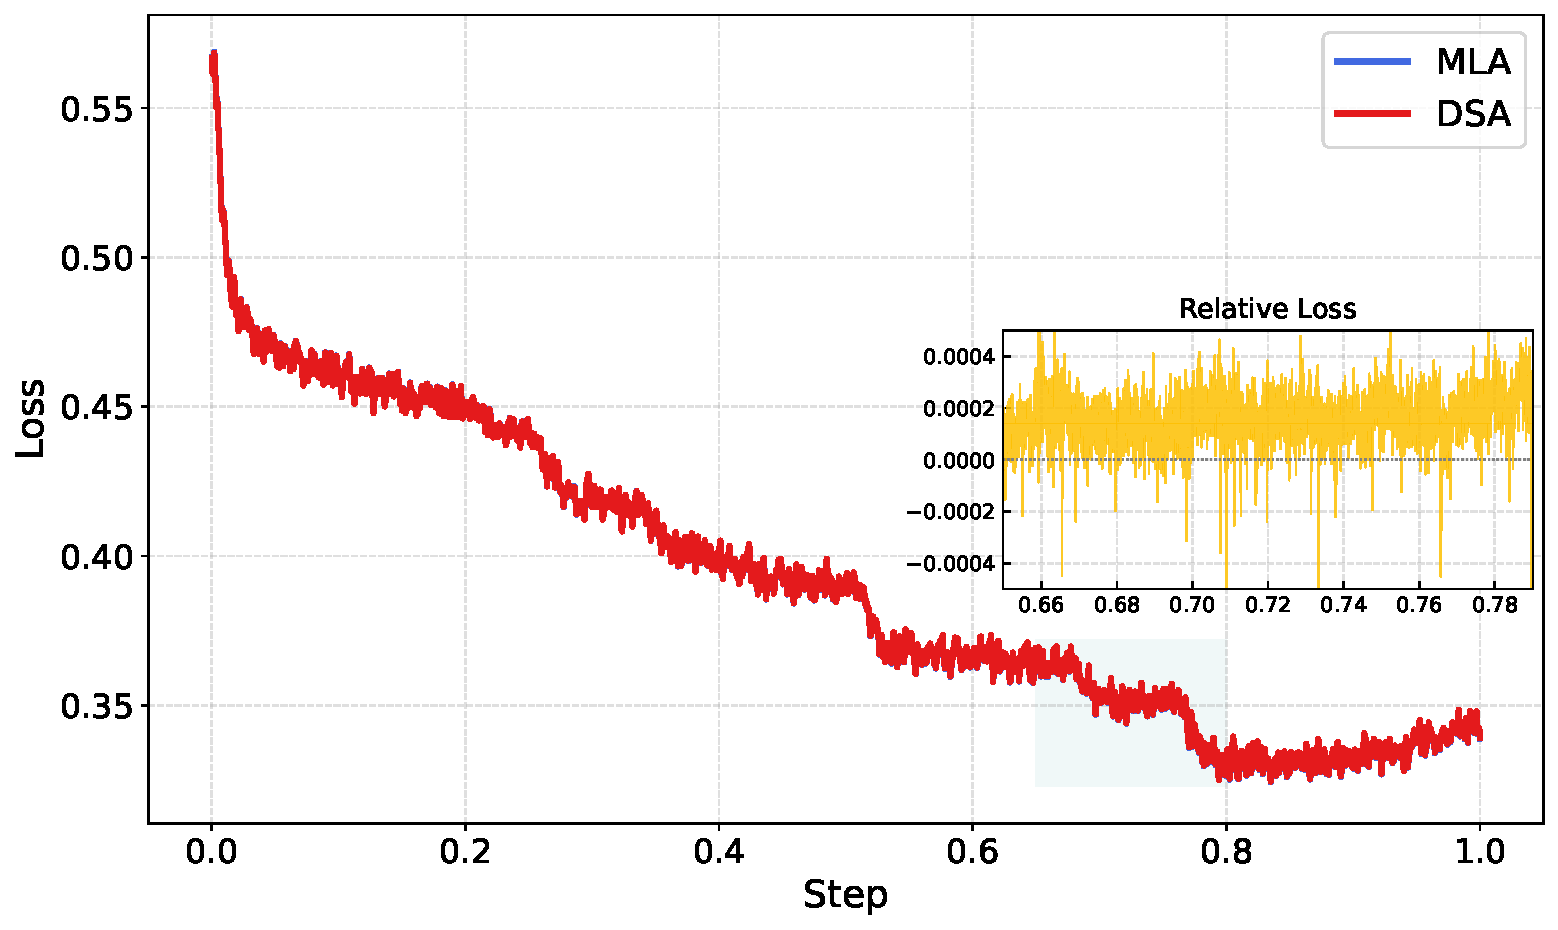
\includegraphics[width=0.6\linewidth]{figures/loss_v2.pdf}
    \caption{SFT loss curves comparison between MLA and DSA training. Results are smoothed by Running Average with a window size of 50.}
    \label{fig:placeholder}
\end{figure}

The DSA training begins from the base model at the end of mid-training. The warm-up stage goes through 1000 steps with each step trained on 14 sequences of 202,752 tokens and a maximum learning rate of 5e-3. The sparse adaptation stage follows the training data and hyperparameters of mid-training and goes through 20B tokens. Although the training budget is much smaller than that of DeepSeek-V3.2 (943.7B tokens), we find that it is enough to adapt the DSA model to match the performance of the original MLA model. As shown in \Cref{tab:dsa}, the long-context performance of the DSA model is close to that of the MLA model. To further validate the effectiveness of DSA training, we fine-tune the DSA and MLA models with the same SFT data, respectively, and find that the two models tie in training loss and evaluation benchmarks.

\subsubsection{Ablation Study of Efficient Attention Variants}

Beyond DSA~\cite{liu2025deepseek}, we explore several alternative efficient attention mechanisms based on GLM-9B\footnote{One of our GLM-4 series models, available at https://github.com/zai-org/GLM-4}. The baseline employs group query attention across all 40 layers and has been fine-tuned with a 128K-token context window. We evaluate the following approaches:

\begin{itemize}[leftmargin=1.5em,itemsep=2pt]
    \item {{Sliding Window Attention (SWA) Interleave:}} A fixed alternating pattern of
    full-attention and windowed-attention layers applied uniformly across the network.
    \item {{Gated DeltaNet (GDN)}~\cite{yanggated}}: A linear attention variant that
    replaces the quadratic softmax attention computation with a gated linear recurrence,
    reducing the computational cost of attention from quadratic to linear in sequence length.
\end{itemize}

\noindent Building on these baselines, we propose two improvements:

\begin{itemize}[leftmargin=1.5em,itemsep=2pt]
    \item {SWA Pattern (Search-Based):} Inspired by PostNAS~\cite{gu2025jet}, we introduce a search-based adaptation method that identifies the optimal subset of layers for SWA conversion while retaining full attention in the remaining layers. We employ a beam search strategy to determine the configuration that maximizes performance on long-context downstream tasks. To mitigate computational costs, we conduct the search exclusively at a 16K context length and generalize the resulting pattern to all other input lengths. Specifically, we use a beam size of~8, optimizing two layers per step; for GLM-9B (40 layers), the process converges in approximately 10 steps. At each step, candidate patterns are evaluated on the RULER benchmark~\cite{hsiehruler} at 16K context length, and the top-8 candidates are retained for the subsequent step. The final derived pattern is \texttt{SFSSFFSSSFFFFSSFSFFFFFFSFSFSSFSSFSFSSFSSS}, where \texttt{S} and \texttt{F} denote SWA and full-attention layers, respectively. As shown in Table~\ref{tab:ruler_results}, this search-based configuration significantly outperforms the fixed interleaved approach. Notably, despite being optimized only at 16K, the pattern exhibits robust length generalization, maintaining effective across all tested context lengths.

    \item {SimpleGDN:} A minimalist linearization strategy designed for maximal reuse of pre-trained weights, improving upon GDN for continual-training adaptation. We remove the \texttt{Conv1d} and explicit gating modules entirely and instead directly map the pre-trained Query, Key, and Value projection weights into the linear recurrence formulation. This simplification eliminates the need for additional parameters while preserving the efficiency benefits of linear attention.
\end{itemize}

\begin{table}[h]
    \small
    \centering
    \caption{RULER benchmark results for the GLM-9B baseline and two SWA variants \emph{without any additional training}. Both SWA methods use a 1:1 ratio of full-attention to SWA layers with a 4096-token window size. The search-based SWA pattern is discovered once at 16k context length and applied uniformly across all input lengths.}
    \label{tab:ruler_results}
    \begin{tabular}{lcccccc}
        \toprule
         & {4K} & {8K} & {16K} & {32K} & {64K} & {128K} \\
        \midrule
        GLM-9B (Full Attn)  & 95.19 & \textbf{93.67} & \textbf{92.01} & \textbf{91.09} & \textbf{85.35} & \textbf{75.28} \\
        SWA Interleave      & 94.87 & 54.02 & 25.89 & 12.61 &  8.32 &  6.51 \\
        SWA Pattern & \textbf{95.78} & 92.54 & 88.92 & 82.52 & 70.23 & 53.95 \\
        \bottomrule
    \end{tabular}
\end{table}

We evaluate all methods on four long-context benchmarks: RULER~\cite{hsiehruler}, MRCR\footnote{\url{https://huggingface.co/datasets/openai/mrcr}}, HELMET-ICL~\cite{yen2024helmet}, and RepoQA~\cite{liu2024repoqa}. Results are summarized in Table~\ref{tab:gqa_results_appendix}. We continually train each method on 190B tokens with a 64K context length, maintaining a 1:1 ratio between efficient attention layers and full attention layers. For the GDN and SimpleGDN methods, we follow the Jet-Nemotron~\cite{gu2025jet} pipeline.

\begin{table*}[h]
\centering
\caption{Long-context benchmark results. All efficient attention variants are continual-trained from the GLM-9B full-attention baseline. SWA pattern denotes search-based layer selection; SWA interleave denotes the fixed alternating pattern. $\Delta$@64K and $\Delta$@128K show the difference relative to the full-attention baseline at 64K and 128K context lengths, respectively.}
\label{tab:gqa_results_appendix}
\resizebox{\textwidth}{!}{
\begin{tabular}{lcccc}
\toprule
  & \textbf{RULER (64K\,/\,128K)}
  & \textbf{MRCR (64K\,/\,128K)}
  & \textbf{HELMET-ICL (64K\,/\,128K)}
  & \textbf{RepoQA (64K\,/\,128K)} \\
\midrule
GLM-9B 
  & 85.35\,/\,75.28
  & 36.53\,/\,35.39
  & 77.68\,/\,77.36
  & 69.00\,/\,65.83 \\
\midrule
SWA Interleave
  & 65.94\,/\,44.93 {\scriptsize($\downarrow$19.41\,/\,$\downarrow$30.35)}
  & 30.03\,/\,28.83 {\scriptsize($\downarrow$6.50\,/\,$\downarrow$6.56)}
  & 75.96\,/\,63.52 {\scriptsize($\downarrow$1.72\,/\,$\downarrow$13.84)}
  & 50.33\,/\,39.33 {\scriptsize($\downarrow$18.67\,/\,$\downarrow$26.50)} \\
SWA Pattern
  & \textbf{83.72\,/\,69.59} {\scriptsize($\downarrow$1.63\,/\,$\downarrow$5.69)}
  & \textbf{35.02\,/\,33.58} {\scriptsize($\downarrow$1.51\,/\,$\downarrow$1.81)}
  & 76.48\,/\,74.60 {\scriptsize($\downarrow$1.20\,/\,$\downarrow$2.76)}
  & 62.33\,/\,51.17 {\scriptsize($\downarrow$6.67\,/\,$\downarrow$14.66)} \\
GDN
  & 76.76\,/\,64.00 {\scriptsize($\downarrow$8.59\,/\,$\downarrow$11.28)}
  & 31.72\,/\,30.22 {\scriptsize($\downarrow$4.81\,/\,$\downarrow$5.17)}
  & 76.88\,/\,74.84 {\scriptsize($\downarrow$0.80\,/\,$\downarrow$2.52)}
  & 65.50\,/\,56.17 {\scriptsize($\downarrow$3.50\,/\,$\downarrow$9.66)} \\
SimpleGDN
  & 81.76\,/\,67.03 {\scriptsize($\downarrow$3.59\,/\,$\downarrow$8.25)}
  & 33.03\,/\,31.27 {\scriptsize($\downarrow$3.50\,/\,$\downarrow$4.12)}
  & \textbf{79.80\,/\,81.84} {\scriptsize($\uparrow$2.12\,/\,$\uparrow$4.48)}
  & \textbf{65.50\,/\,58.50} {\scriptsize($\downarrow$3.50\,/\,$\downarrow$7.33)} \\
\bottomrule
\end{tabular}
}
\end{table*}

The results in Table~\ref{tab:gqa_results_appendix} reveal a clear trade-off hierarchy among efficient attention methods. Naively interleaved sliding window attention (SWA) causes catastrophic degradation on long-context tasks (e.g., $-$30.35 on RULER@128K), while search-based layer selection substantially narrows this gap by preserving full attention where it matters most. Linear attention variants such as GDN further improve quality but at the cost of additional parameters; SimpleGDN strikes the best balance by maximally reusing pre-trained weights. Nevertheless, all of these methods incur an inherent accuracy gap on fine-grained retrieval tasks—up to 5.69 points on RULER@128K and 7.33 on RepoQA@128K—due to the unavoidable information loss introduced by efficient attention mechanisms during continual-training adaptation, even when half of the layers retain full attention. In contrast, DSA is lossless by construction: its lightning indexer achieves token-level sparsity without discarding any long-range dependencies, enabling application to all layers with no quality degradation.


To verify this, we conduct a small-scale DSA experiment on GLM-4.7-Flash\footnote{\url{https://huggingface.co/zai-org/GLM-4.7-Flash}} with multi-latent attention. Following the standard DSA recipe, training proceeds in two stages: (i)~a {warmup} phase that trains only the indexer for 1{,}000 steps (batch size 16) while keeping all base-model weights frozen, followed by (ii)~a {joint-training} phase in which both the model and the indexer are co-trained on 150B tokens.
Table~\ref{tab:dsa_ruler_results} summarizes the results on RULER across context lengths from 4K to 128K. Even the warmup-only variant ({GLM-4.7-Flash + DSA warmup}) already preserves the vast majority of baseline performance; the drop is modest and concentrated at the longest context window (128K: $79.21 \to 71.35$), while shorter contexts remain virtually unaffected. After the full 150B-token joint-training phase, {GLM-4.7-Flash + DSA} closes nearly all of this residual gap: it {surpasses} the baseline at 16K ($+0.86$), 32K ($+0.49$), and 64K ($+1.72$), while incurring only a 0.35-point deficit at 128K.

\begin{table}[t]
    \small
    \centering
    \caption{RULER benchmark results for the GLM-4.7-Flash with DSA.
    The warmup-only variant trains only the indexer while
    keeping the base model frozen, the full DSA variant jointly trains both for
    150B tokens. }
   \label{tab:dsa_ruler_results}
    \begin{tabular}{lcccccc}
        \toprule
         & {4K} & {8K} & {16K} & {32K} & {64K} & {128K} \\
        \midrule
        GLM-4.7-Flash  & 97.44 & 96.72 & 95.83 & 92.96 & 85.34 & 79.21 \\
        GLM-4.7-Flash + DSA warmup & 97.51 & 96.54 & 95.40 & 90.09 & 84.05 & 71.35  \\
        GLM-4.7-Flash + DSA & 96.77 & 96.25 & 96.69 & 93.45 & 87.06 & 78.86 \\
        \bottomrule
    \end{tabular}
\end{table}



\subsection{Pre-training Data}

\paragraph{Web.} Building upon the GLM-4.5 data pipeline, we refined our selection criteria for massive web datasets. We introduced another DCLM~\cite{li2025datacomplmsearchgenerationtraining} classifier based on sentence embeddings to identify and aggregate additional high-quality data beyond standard classifiers. To address the challenge of long-tail knowledge, we utilized a World Knowledge classifier—optimized via Wikipedia entries and LLM-labeled data—to distill valuable information from otherwise medium-low-quality data.

\paragraph{Code.} We expand the code pre-training corpus with refreshed snapshots from major code hosting platforms and a larger collection of code-containing web pages, resulting in a 28\% increase in fuzzily deduplicated unique tokens. To improve corpus integrity and reduce noise, we fix metadata alignment issues in Software Heritage code files and adopt a more accurate language classification pipeline. We follow GLM-4.5’s quality-aware sampling strategy for source code and code-related web documents. In addition, we train dedicated classifiers for a broader set of low-resource programming languages (e.g., Scala, Swift, Lua, etc.), improving sampling quality for these languages.

\paragraph{Math \& Science.} We collect high-quality math \& science data from webpages, books, and papers to further increase the reasoning abilities. Specifically, the content extraction pipelines for webpages and PDF parsing mechanisms
for books and papers are refined to increase data quality. We adopt large language models to score candidate documents and only retain the most educational content. For long-context documents, we develop a chunk-and-aggregate scoring algorithm to increase scoring accuracy. Filtering pipelines are conducted to strictly avoid the use of synthetic, AI-generated, or template-based data. 



\subsection{Mid-Training}

Building upon the mid-training framework introduced in GLM-4.5, we scale up both the training volume and the maximum context length in GLM-5 to further strengthen the model's reasoning, long-context, and agentic capabilities.

\paragraph{Extended context and training scale.} We progressively extend the context window across three stages: 32K (1T tokens), 128K (500B tokens), and 200K (50B tokens). Compared to the 128K maximum in GLM-4.5, the additional 200K stage substantially improves the model's ability to process ultra-long documents and complex multi-file codebases. Long documents and synthetic agent trajectories are up-sampled at the later stages accordingly.

\paragraph{Software engineering data.} We retain the paradigm of concatenating repo-level code files, commit diffs, GitHub issues, pull requests, and relevant source files into unified training sequences. In GLM-5, we relax the repository-level filtering criteria to broaden the pool of eligible repositories, yielding approximately 10 million issue–PR pairs, while strengthening quality filtering at the individual issue level to reduce noise. We also retrieve a larger set of relevant files for each issue–PR pair, resulting in richer development contexts and broader coverage of real-world software engineering scenarios. After filtering, the issue–PR portion of the dataset comprises approximately 160B unique tokens.

\paragraph{Long-context data.} Our long-context training set comprises both natural and synthetic data. Natural data is curated from books, academic papers, and documents from general pre-training corpora employing multi-stage filtering (PPL, deduplication, length) and upsampling knowledge-intensive domains. In synthetic data construction, inspired by NextLong\cite{gao2025nextlongeffectivelongcontexttraining} and EntropyLong\cite{jia2025entropylongeffectivelongcontexttraining}, we employed diverse techniques to build long-range dependencies. Highly similar texts were aggregated via interleaved packing to produce sequences, aiming to mitigate the lost-in-the-middle phenomenon and improve performance across a range of long-context tasks. At the 200K stage, we additionally incorporated a small proportion of MRCR-like data, with multiple variants designed to extend OpenAI's original paradigm, to strengthen recall in extended multi-turn dialogues. Empirically, we find that increasing data diversity progressively enhances the model's long-context performance; notably, a subsequent 200K mid-training stage, building upon the initial 128K phase, further bolstered the model’s performance even within the 128K context window.

\subsection{Training Infrastructure}

\subsubsection{Memory Efficiency}

\textbf{Flexible MTP placement.} Under interleaved pipeline parallelism~\cite{narayanan2021efficientlargescalelanguagemodel}, model components are flexibly assigned to stages. The MTP module spans embedding, transformer, and output components. It incurs substantially higher memory usage than other modules, leading to stage-level imbalance. We co-locate the MTP output layer with the main output layer on the final stage to enable parameter sharing, while placing its embedding and transformer components on the preceding stage. This reduces memory pressure on the final stage and improves balance across pipeline ranks.

\textbf{Pipeline ZeRO2 gradient sharding.} Each pipeline rank maintains multiple stages~\cite{narayanan2021efficientlargescalelanguagemodel}, and naively each stage requires a full gradient buffer for accumulation and optimizer updates. Inspired by ZeRO2~\cite{rajbhandari2020zeromemoryoptimizationstraining}, we shard gradients across data-parallel ranks so that each stage stores only a 1/dp fraction of the full gradients. In addition, we retain full accumulation buffers for only two stages at a time and reuse them via double buffering. While one stage buffer accumulates gradients over consecutive microbatches, gradient synchronization for the previous stage buffer is performed in parallel. This reduces persistent gradient memory to per-stage sharded buffers plus only two full buffers for rolling accumulation, without additional synchronization overhead in practice.

\textbf{Zero-redundant communication for the Muon distributed optimizer.} Naive Muon implementations all-gather full model parameters on each data-parallel rank, causing transient memory spikes and redundant communication. We restrict all-gather to parameter shards owned by each rank and overlap local computation with shard communication. This eliminates redundant communication and significantly reduces optimizer-related peak memory overhead.

\textbf{Pipeline activation offloading.} During pipeline warmup, forward execution advances ahead of backpropagation, prolonging the lifetime of intermediate activations. We offload the activations to host memory after forward execution and reload them prior to backward execution~\cite{298555}. Offloading is applied at layer granularity to further reduce peak memory usage. Combined with fine-grained recomputation, this largely eliminates the need to keep activations resident in GPU memory. Offload and reload are scheduled to overlap with computation while avoiding contention with peer-to-peer communication and MoE token routing (dispatch and combination). This substantially reduces the activation memory footprint with near-zero overhead.

\textbf{Sequence-chunked output projection for peak memory reduction.} 
Output projection and cross-entropy loss incur transient memory overhead from storing activations for backpropagation and promoting them to higher precision during loss computation. To reduce this overhead, we partition the input sequence into smaller chunks and compute projection and loss independently on each chunk, completing forward and backward passes and releasing activations before moving on. As a result, peak memory usage decreases as the number of chunks increases. With an appropriate chunk count, this approach alleviates output-layer memory pressure while maintaining performance comparable to unchunked execution.


\subsubsection{Parallelism Efficiency}

\textbf{Efficient deferred weight gradient computation.} To reduce pipeline bubbles, we defer some weight gradient computation of the critical path~\cite{qi2023zero}. Fine-grained deferral with optimized storage and communication overlap improves throughput while keeping memory overhead bounded.

\textbf{Efficient long-sequence training.} Longer sequences exacerbate load imbalance across data parallel and pipeline parallel groups. We address this through workload-aware sequence reordering, dynamic redistribution of attention computation, and flexible partitioning of data parallel ranks into context-parallel groups of varying sizes~\cite{ge2025bytescale,wang2025flexsp}. A hierarchical all-to-all overlaps intra-node and inter-node communication for QKV tensors to reduce latency.

\subsubsection{INT4 Quantization-aware training}

To provide better accuracy at low-precision, we apply INT4 QAT in the SFT stage. Moreover, to further mitigate the training time overhead, we have developed a quantization kernel applicable to both training and offline weight quantization, which ensures bitwise-identical behavior between training and inference.
